\documentclass{article}
\textheight 20.5truecm \textwidth 14.5truecm
\setlength{\oddsidemargin}{0.35in}\setlength{\evensidemargin}{0.35in}

\usepackage[utf8]{inputenc}
\usepackage[russian]{babel}
\usepackage{graphicx}
\usepackage{amsmath}
\usepackage{breqn}
\usepackage{wrapfig}
\usepackage{float}
\usepackage{multirow}
\usepackage{caption}
\usepackage{subcaption}

\graphicspath{ {./data/images} }
\author{Александр Романов Б01-110}
\date{}
\title{4.2. Исследование энергетического спектра \(\beta\)-частиц и определение их
максимальной энергии при помощи магнитного спектрометра}

\begin{document}
\maketitle
\section{Введение}
\subsection{Краткое описание}
С помощью магнитного спектрометра исследуется энергетический спектр \(\beta\)-частиц
при распаде ядер \(\text{Cs}^{137}\) и определяется их максимальная энергия. Калибровка
спектрометра осуществляется по энергии электронов внутренней конверсии \(\text{Cs}^{137}\)
\subsection{Экспериментальная установка}

\begin{figure}[H]
	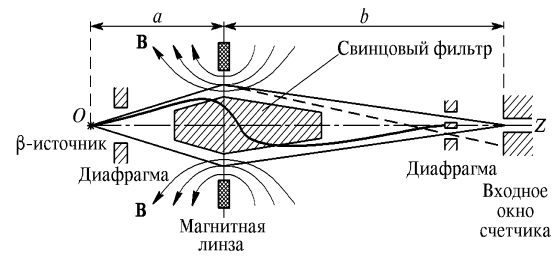
\includegraphics[width=\textwidth]{scheme.png}
	\caption{Схема \(\beta\)-спектрометра с короткой магнитной линзой}
\end{figure}

\begin{figure}[H]
	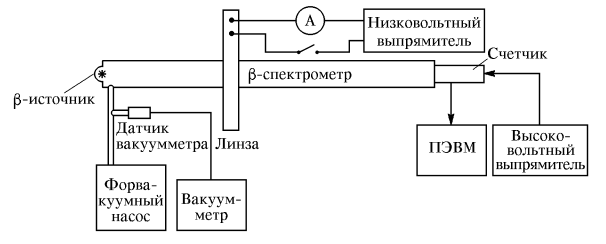
\includegraphics[width=\textwidth]{scheme-2.png}
	\caption{Блок-схема установки}
\end{figure}


\section{Работа}

Откачаем воздух из полости спектрометра. Включим вакуумметр. Включим формироватлель
инпульсов, питание магнитной линзы и уменьшим ток через неё до нуля. Запустим измерение
спектра в программе на ПЭВМ длительностью в 100с. Будем измерять с шагом тока через катушку равным 0.2A.

\begin{table}[h]
	\centering
\begin{tabular}{|c|c|}
\hline
I, A & N    \\\hline
0.00 & 438  \\\hline
0.00 & 129  \\\hline
0.00 & 119  \\\hline
0.20 & 114  \\\hline
0.40 & 136  \\\hline
0.60 & 150  \\\hline
0.80 & 273  \\\hline
1.00 & 556  \\\hline
1.20 & 929  \\\hline
1.40 & 1189 \\\hline
1.60 & 1394 \\\hline
1.80 & 1489 \\\hline
2.00 & 1496 \\\hline
2.20 & 1449 \\\hline
2.40 & 1089 \\\hline
2.60 & 792  \\\hline
2.80 & 396  \\\hline
3.00 & 422  \\\hline
3.10 & 1276 \\\hline
3.15 & 1935 \\\hline
3.20 & 2279 \\\hline
3.25 & 2447 \\\hline
3.30 & 2229 \\\hline
3.35 & 1759 \\\hline
3.40 & 1487 \\\hline
3.50 & 602  \\\hline
3.60 & 265  \\\hline
3.78 & 82   \\\hline
4.00 & 80   \\\hline
4.20 & 57   \\\hline 
\end{tabular}
	\caption{Результаты измерения числа \(N\) от тока на катушке \(I\) (\(t = 100s\))}
\end{table}
Изобразим это графически:

\begin{figure}[H]
	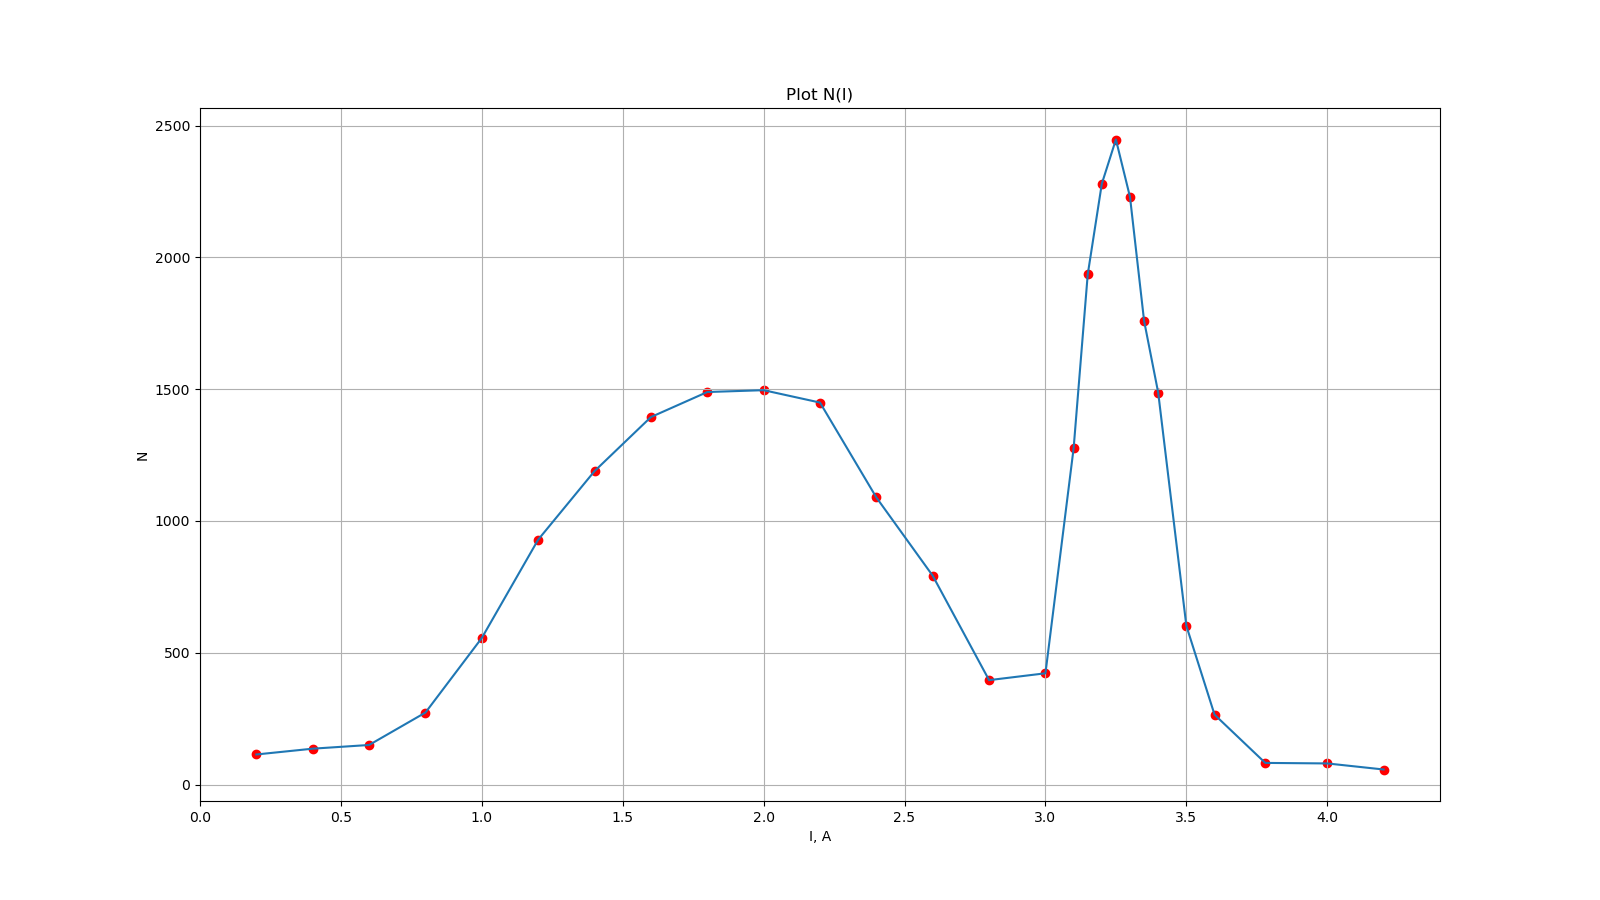
\includegraphics[width=\textwidth]{I-N.png}
\end{figure}

Вспомним следующую формулу:
\[ \frac{\sqrt{N(p)/t}}{p} \simeq E_e - E \]

Проведём преобразования наших данных и построим график \(\frac{\sqrt{N/t}}{I}\) от \(I\)
(график Ферми-Кюри):

\begin{figure}[H]
	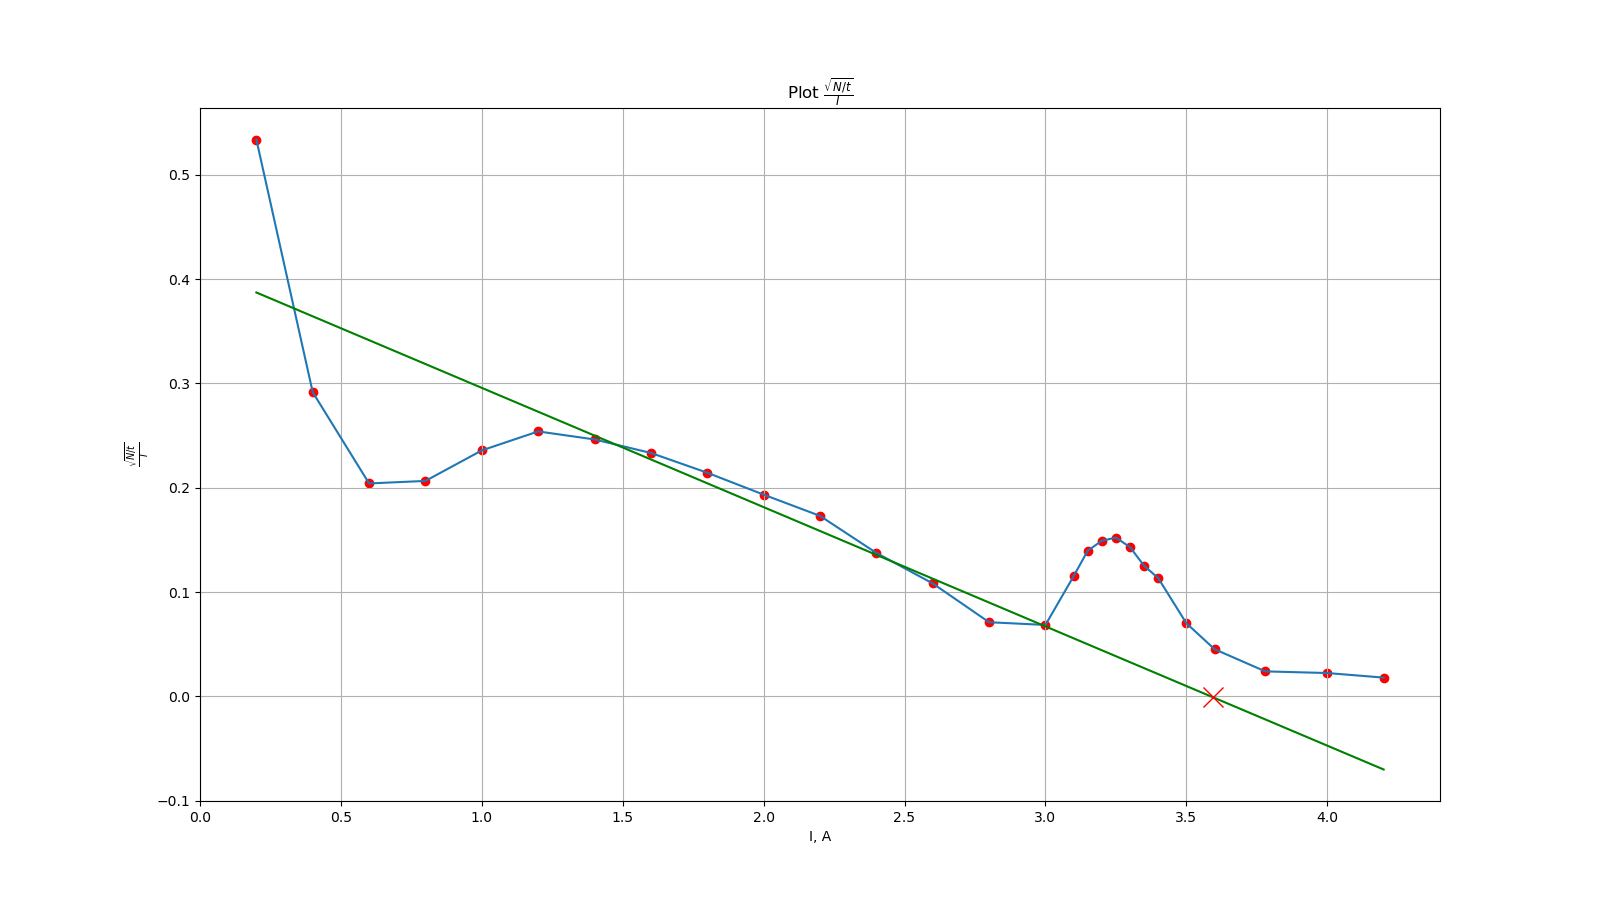
\includegraphics[width=\textwidth]{I-Nr.png}
	\caption{График Ферми-Кюри}
\end{figure}

Аппроксимируем график прямой на линейном участке:

\[ \frac{\sqrt{N/t}}{I} = (-0.114 \pm 0.006) * I + (0.410 \pm 0.09)\]

По пересечению линии с осью абсцисс определим \(E_e\):
\[ E_e = 0.045 \pm 0.006 MeV\]

\section{Выводы}
В результате выполнения работы:
\begin{enumerate}
	\item Был изучен \(\beta\)-спектр при распаде ядра \(\text{Cs}^{137}\)
	\item Был получен и исследован график Ферми-Кюри и получено значение энергии \(E_e = 0.045 \pm 0.006\)
\end{enumerate}

\end{document}
